\documentclass[12pt,a4paper]{article}
\usepackage[utf8]{inputenc}
\usepackage[margin=1in]{geometry}
\usepackage{graphicx}
\usepackage{tabularx}
\usepackage[onehalfspacing]{setspace}
\usepackage{float}
\usepackage[bf]{caption}
\newcommand\fnote[1]{\captionsetup{font=footnotesize}\caption*{#1}}
\usepackage{booktabs}

\title{Results}
\author{SoDa Labs}
\date{October 2025}

\begin{document}

\maketitle

\section{Summary Statistics}

\begin{table}[H]
\centering
\caption{Summary Statistics}
\label{tab:summary_statistics}
\begin{tabularx}{\textwidth}{Xccc}
\toprule \toprule
Statistic & Precipitation & Temperature & Population \\
\midrule
Mean & 31.00 & 26.00 & 370.48 \\
Standard Deviation & 1.00 & 6.56 & 166.27 \\
Min & 30.00 & 20.00 & 252.65 \\
Max & 32.00 & 33.00 & 560.67 \\
\bottomrule
\end{tabularx}
\end{table}


\begin{figure}
  \centering
  \caption{Precipitation and Population}
  \label{fig:precipitation_population}
  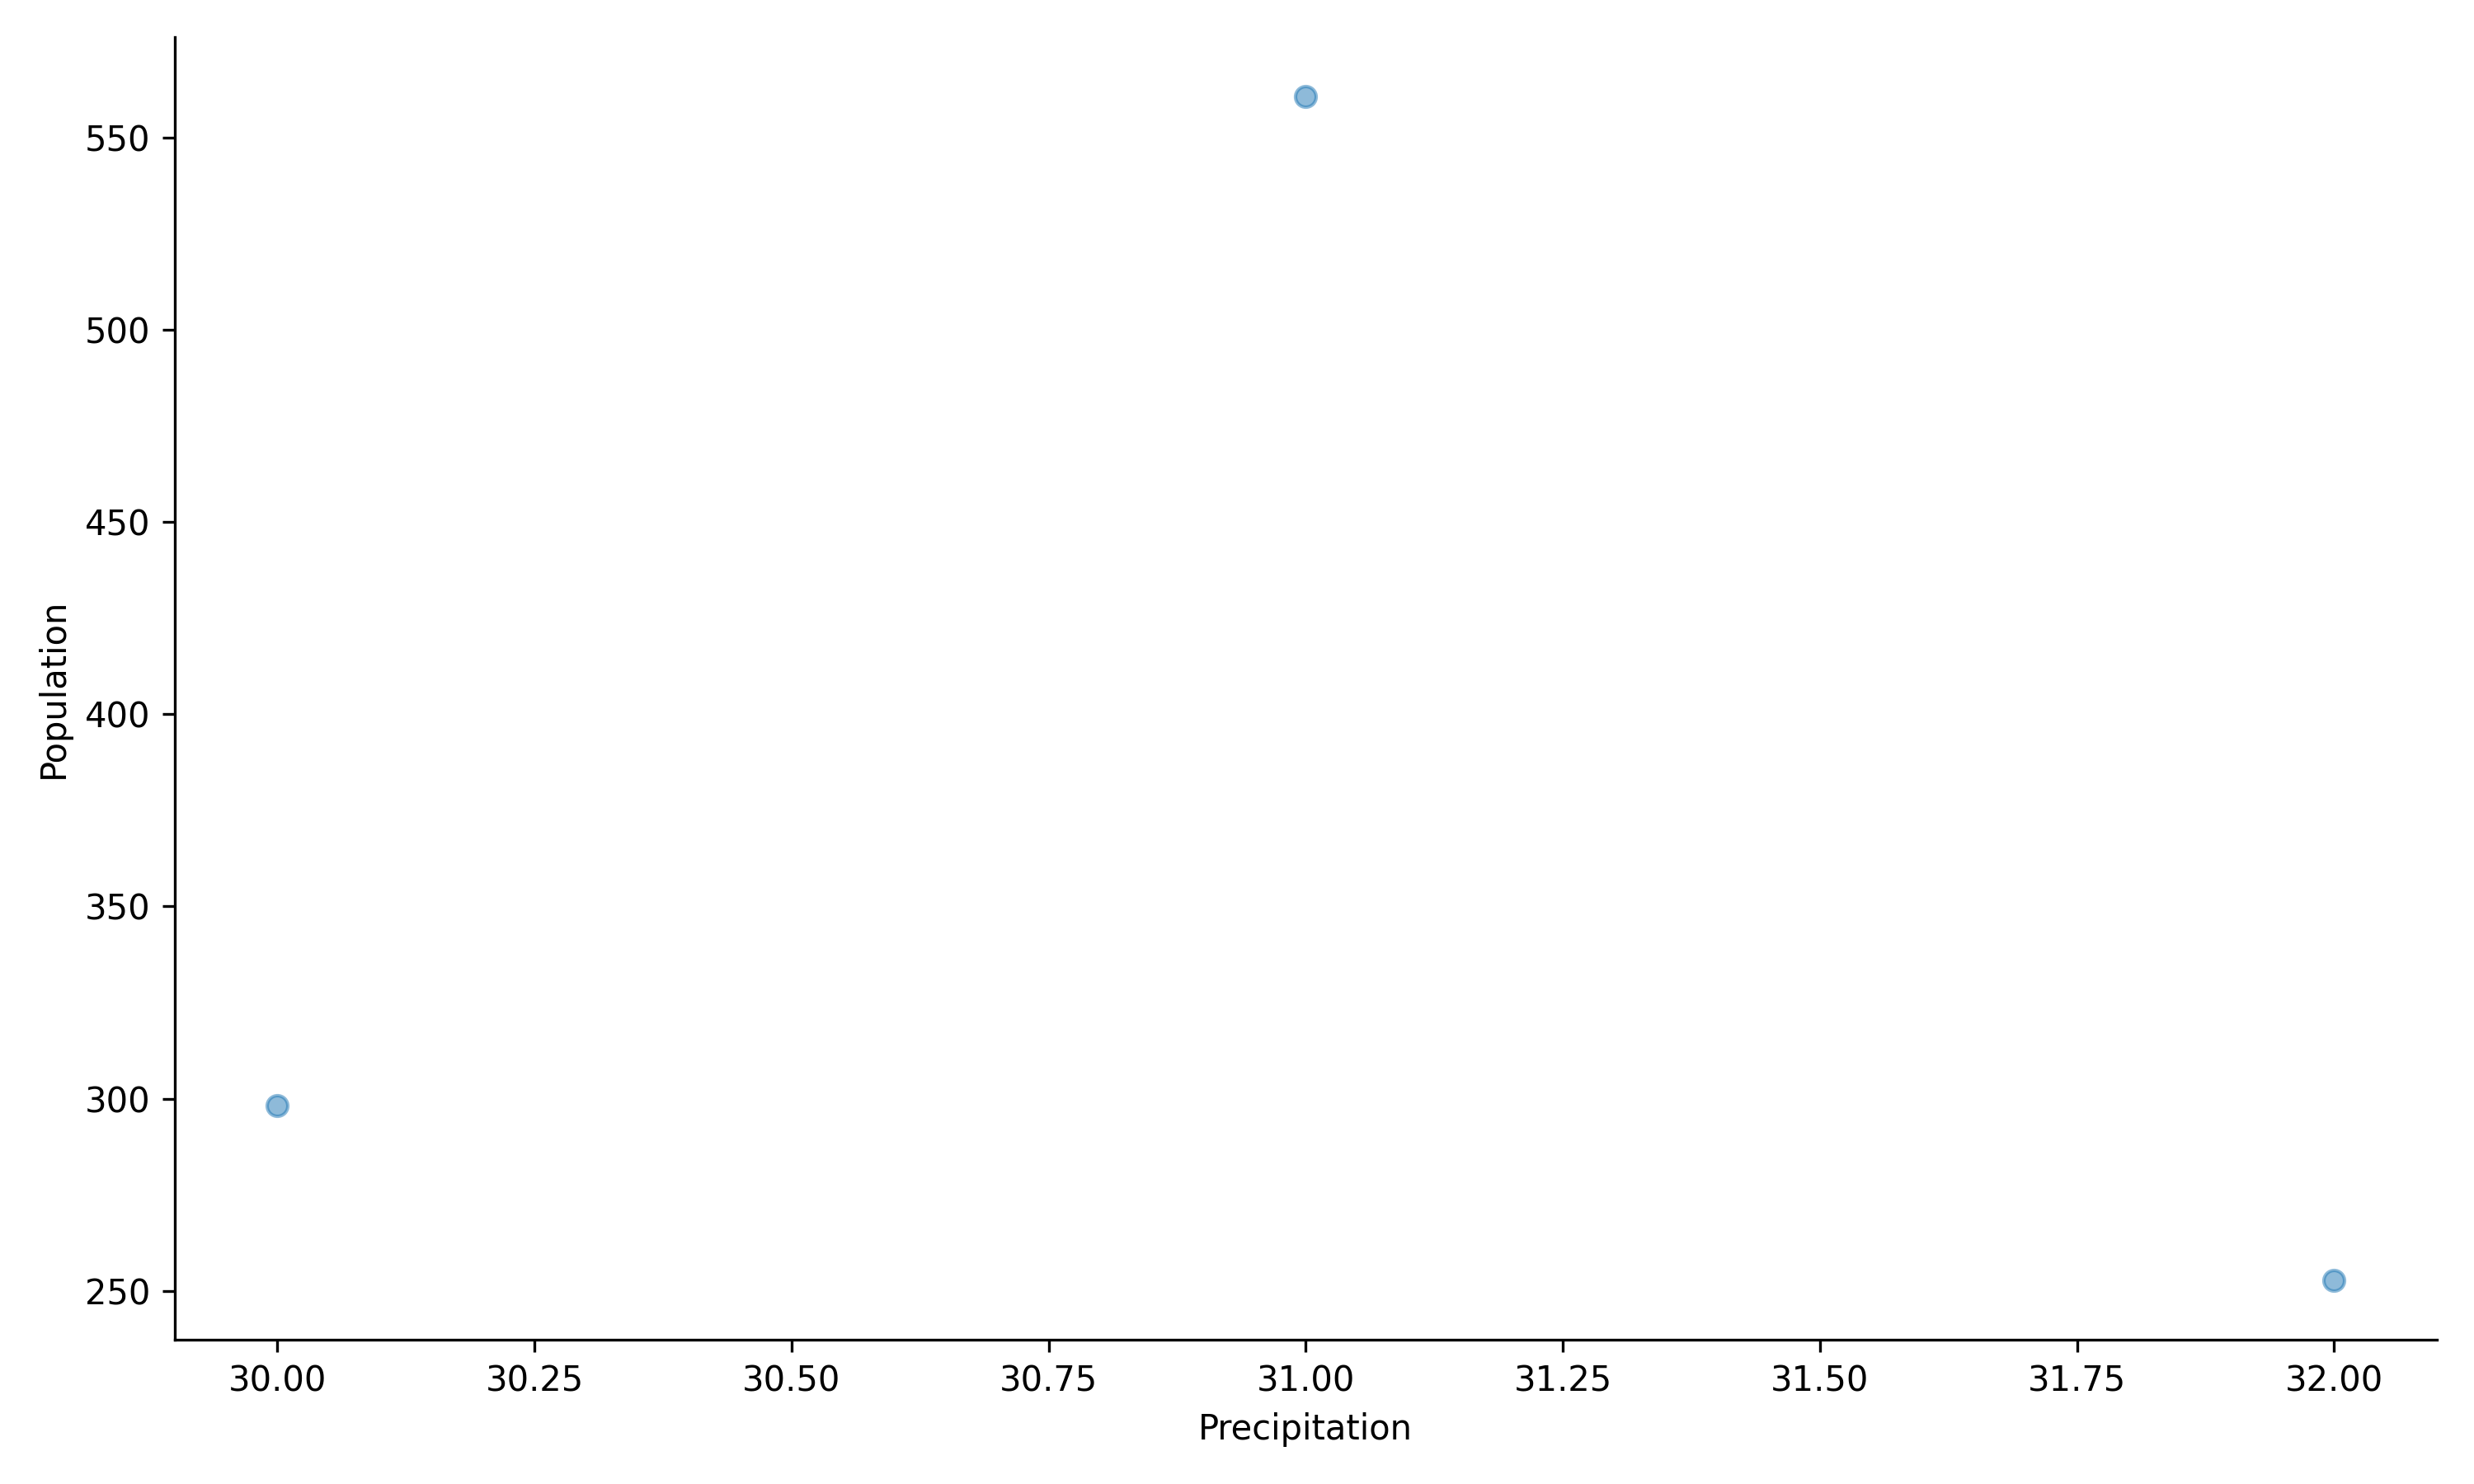
\includegraphics[width=\textwidth]{figures/precipitation_population.png}
\fnote{\scriptsize \textit{Notes:} Precipitation and population of Australian cities.}
\end{figure}

\begin{figure}
  \centering
  \caption{Temperature and Population}
  \label{fig:temperature_population}
  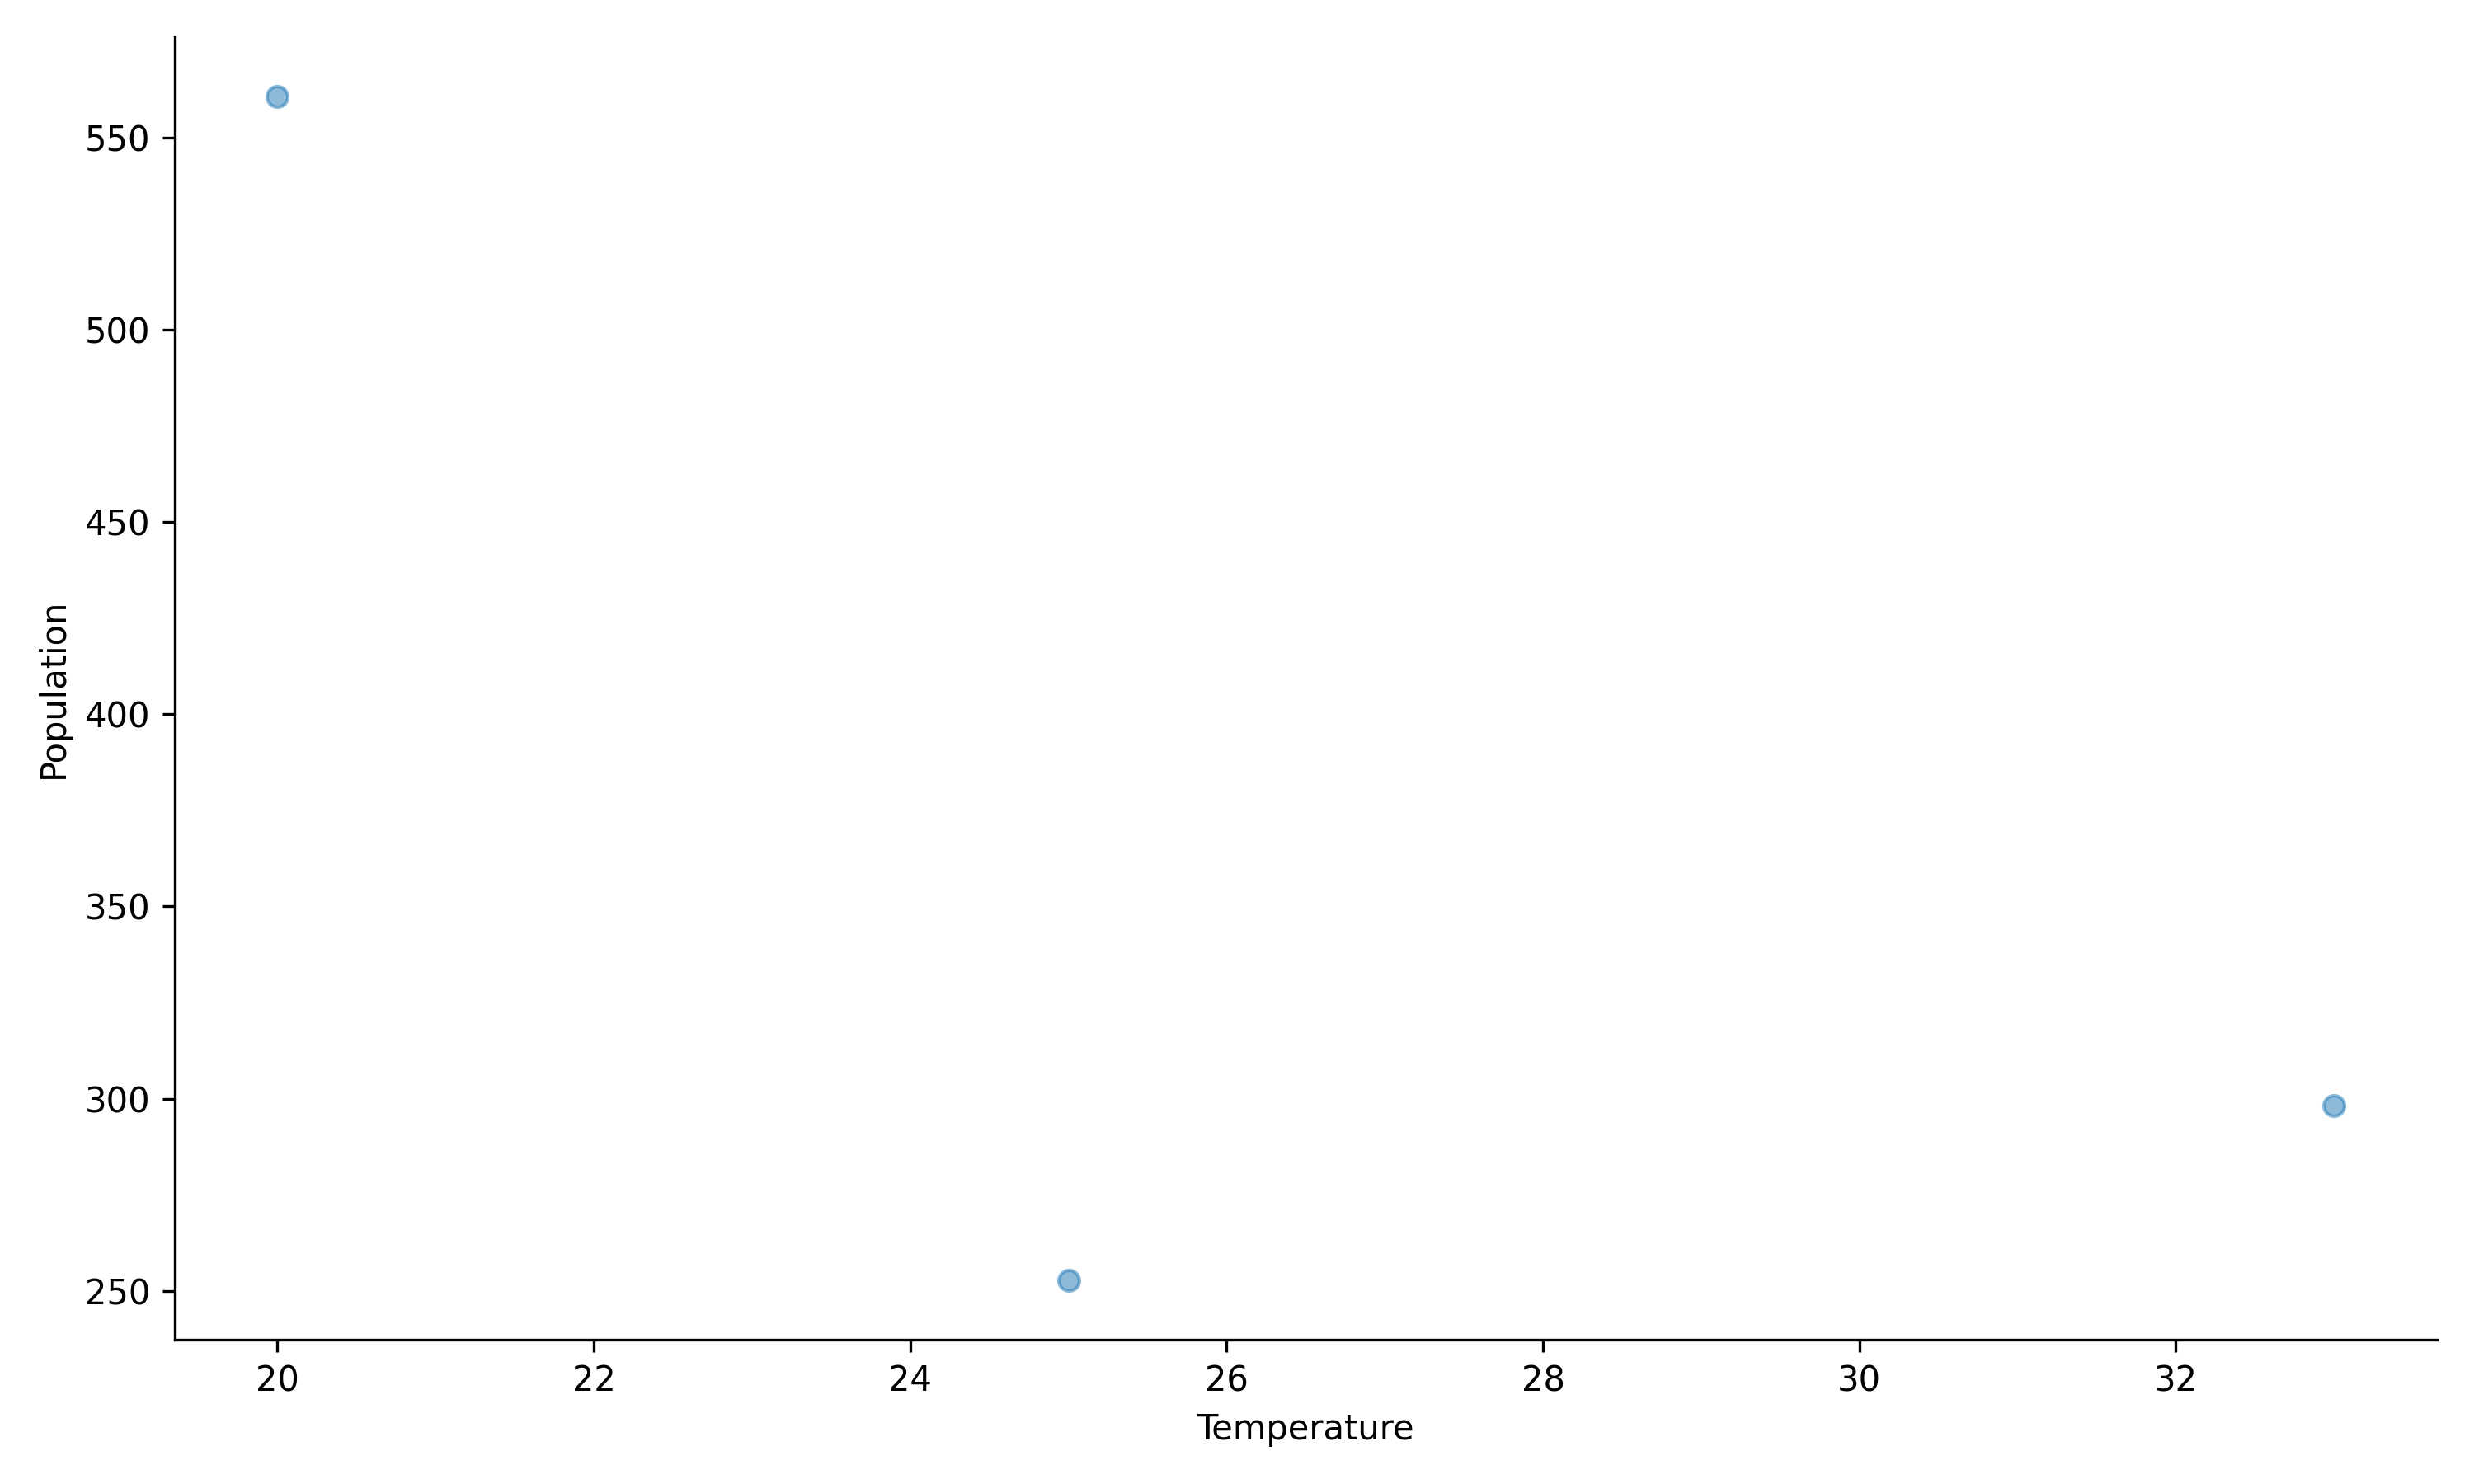
\includegraphics[width=\textwidth]{figures/temperature_population.png}
\fnote{\scriptsize \textit{Notes:} Temperature and population of Australian cities.}
\end{figure}

\end{document}
